\section{Convolution}
This section introduces convolution from a more mathematical perspective and then gives some less traditional applications of a more generalised version.

\subsection{Definition}
Conceptually, the convolution operation gives the overlap between two functions as a function of the offset between the functions.

Mathematically, convolution is defined by an integral \cite{convolution1}:

\[
    (f * g)(t) = \int^{\infty}_{-\infty}{f(\tau)g(t-\tau) d\tau}
\]

The discrete counterpart to this is \cite{convolution2}:

\[
    (f * g)(n) = \sum^{\infty}_{i=-\infty}{f(i)g(n-i)}
\]

This discrete variant is visualised in Figure \ref{fig:VisualConvolution} where only three of the values in the input functions have been highlighted.
Notice how the corresponding values from the input functions are multiplied before the products are summed.

\begin{figure}
    \centering
    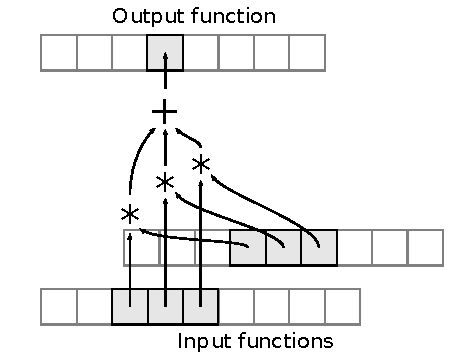
\includegraphics{img/VisualConvolution}
    \caption[Convolution performed on discrete functions]{
        Convolution performed on discrete functions.
        Each box represent a discrete value.
    }
    \label{fig:VisualConvolution}
\end{figure}

Convolution can also be extended to multiple dimensions by summing across the additional dimensions.
For the discrete case, a two-dimensional convolution is expressed as \cite{convolution2}:

\[
    (f * g)(n, m) = \sum^{\infty}_{i=-\infty}\sum^{\infty}_{j=-\infty}{f(i, j)g(n-i, m-j)}
\]

\subsection{Application in Image Processing}
As mentioned in the introduction, convolution can be used in image processing to apply various filters to an image.

A monochrome image can be thought of as a 2D matrix with a width $W$ and height $H$.
The operation to be performed on the image matrix can be expressed as another matrix called the \textit{kernel}.
Let $I(x, y)$ be a function for accessing a specific value in the image matrix.
Let $K(x, y)$ be a function for accessing a specific value in the kernel,
or $0$ if $x$ or $y$ is out of bounds for the kernel matrix.

The convolution of the image and the kernel is then given by
\[
    C(x, y) = \sum^{H}_{h=0} \sum^{W}_{w=0}{I(w, h)K(w - x, h - y)}
\]
where $C(x, y)$ is the output image.
Because $K(w - x, h - y)$ is $0$ for most $w, h$, the resulting values are determined by only a small \textit{neighbourhood} part of the input matrix around $x, y$.

For a coloured image, convolution can be performed once per colour channel. The convolved channels can then be put together again to produce a convolved coloured image.

Depending on the kernel matrix, various effects like blurring or sharpening may be applied to the image with convolution.
A small selection of possible kernel matrices and the results when applied to the image in Figure \ref{fig:LenaOriginal} can be found in Table \ref{tab:KernelMatrices}.

\begin{table}
    \centering
    \begin{tabular}{ccm{3cm}}
    Description & Matrix & Result \\
    \hline
    Blur & $
            \begin{bmatrix}
            1/9 & 1/9 & 1/9 \\
            1/9 & 1/9 & 1/9 \\
            1/9 & 1/9 & 1/9
            \end{bmatrix}
        $ & 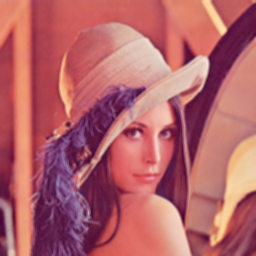
\includegraphics[width=3cm]{img/LenaBlurred} \\
    Edge-detect & $
            \begin{bmatrix}
            -1 & -1 & -1 \\
            -1 & 8 & -1 \\
            -1 & -1 & -1
            \end{bmatrix}
        $ & 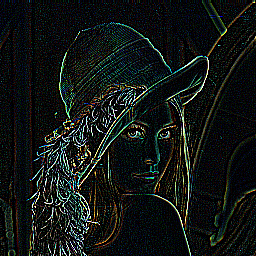
\includegraphics[width=3cm]{img/LenaEdge} \\
    Emboss & $
            \begin{bmatrix}
            -2 & -1 & 0 \\
            -1 & 1 & 1 \\
            0 & 1 & 2
            \end{bmatrix}
        $ & 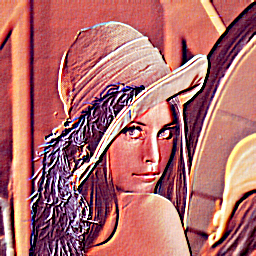
\includegraphics[width=3cm]{img/LenaEmbossed}
    \end{tabular}
    \caption{Some kernels used in image processing}
    \label{tab:KernelMatrices}
\end{table}

As the matrices in Table \ref{tab:KernelMatrices} are good examples of, the kernel matrices used for image processing are usually small compared to the images, and often of a constant size.
This means each output pixel is a function of the same pixel in the original image and its neighbourhood.

\subsection{Generalised Convolution}
The convolution described above can be separated into two stages: first multiplication, then a summation.
The multiplication stage simply maps a set of input values to a set of output values by using the kernel matrix values as factors.
These products are then reduced into a single value by summation.

By recognising that the process consists of a map and a reduce operation,
it becomes possible to substitute the operations with other map and reduce operations.
A generalised convolution operation is therefore fully defined by two input matrices and two operations.

In the realm of image processing, this paves the way for new filters, such as the median, minimum and maximum filters.
These filters are commonly used to remove noise in images and consists of a convolution kernel matrix of ones (the multiplicative identity for scalars),
the multiplication operation for the map stage and the minimum, maximum or mean operations respectively for the reduce operations.
The resulting images created by applying the effect to the \textit{Lena} test image can be seen in Table \ref{tab:GeneralisedKernelMatrices}.

\begin{table}
    \centering
    \begin{tabular}{lm{3cm}}
        Reduce operation & Result \\
        \hline
        Minimum & 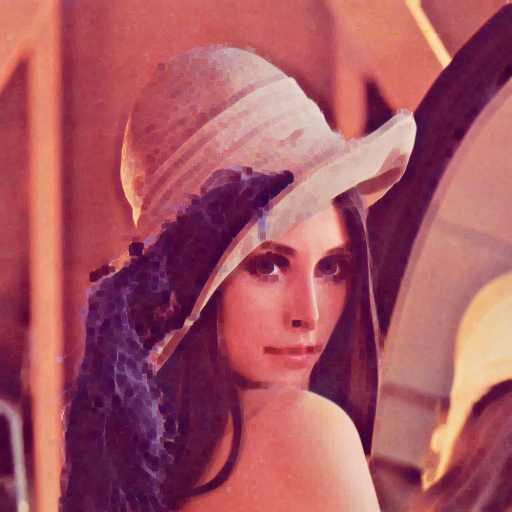
\includegraphics[width=3cm]{img/LenaMin} \\
        Maximum & 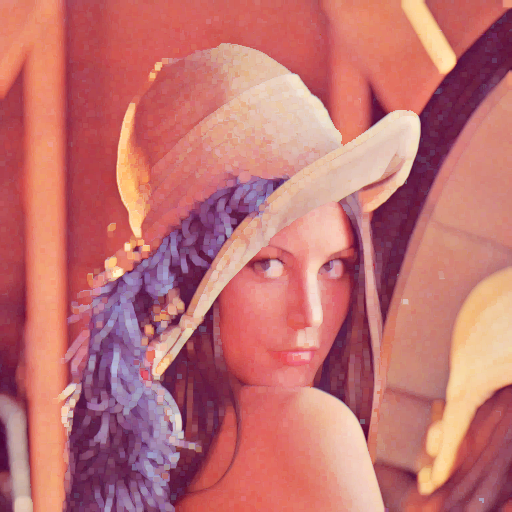
\includegraphics[width=3cm]{img/LenaMax} \\
        Median & 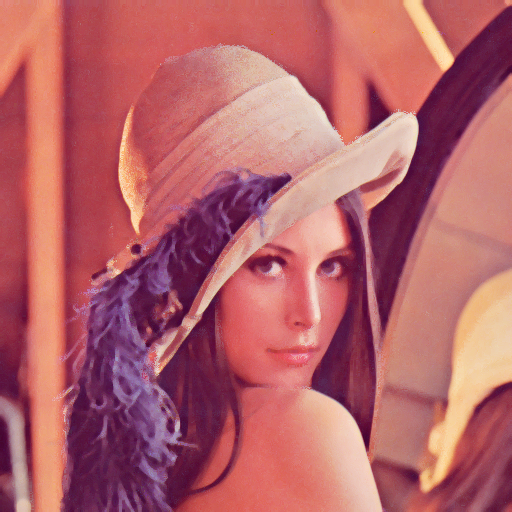
\includegraphics[width=3cm]{img/LenaMedian}
    \end{tabular}

    \caption{Some image processing filters using a generalised form of convolution}
    \label{tab:GeneralisedKernelMatrices}
\end{table}

Generalised convolution can also be used in other areas, such as to calculate the next iteration of cellular automatons. This requires a more advanced reduce operation.
